\section{Рабочий проект}

\subsection{Реализация модуля авторизации и регистрации}

Модуль авторизации и регистрации реализован с использованием SharedPreferences для хранения данных пользователя. При регистрации система проверяет, не зарегистрирован ли уже указанный адрес электронной почты. Если пользователь с таким email не найден, данные сохраняются, и выполняется автоматический вход. При авторизации система сверяет введённые данные с сохранёнными.

На рисунке \ref{fig:auth} представлен экран авторизации и регистрации.

\begin{figure}[H]
	\centering
	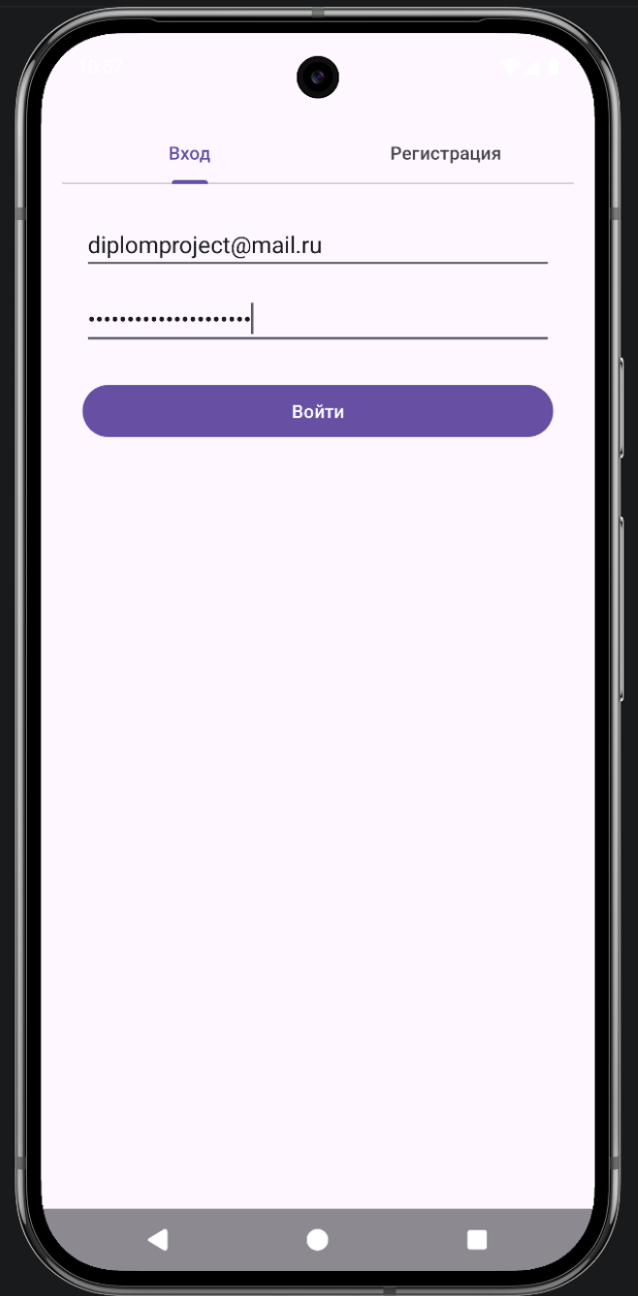
\includegraphics[width=0.4\textwidth]{images/auth.png}
	\caption{Экран авторизации}
	\label{fig:auth}
\end{figure}

\vspace{0.5cm}

\subsection{Реализация каталога занятий}

Каталог занятий реализован с использованием RecyclerView. Данные о занятиях хранятся в SharedPreferences в виде JSON-строк. При загрузке каталога система парсит данные и отображает карточки занятий. Фильтрация по городу реализована на клиентской стороне без дополнительных запросов к хранилищу.

На рисунке \ref{fig:classes} представлен экран каталога занятий.

\begin{figure}[H]
	\centering
	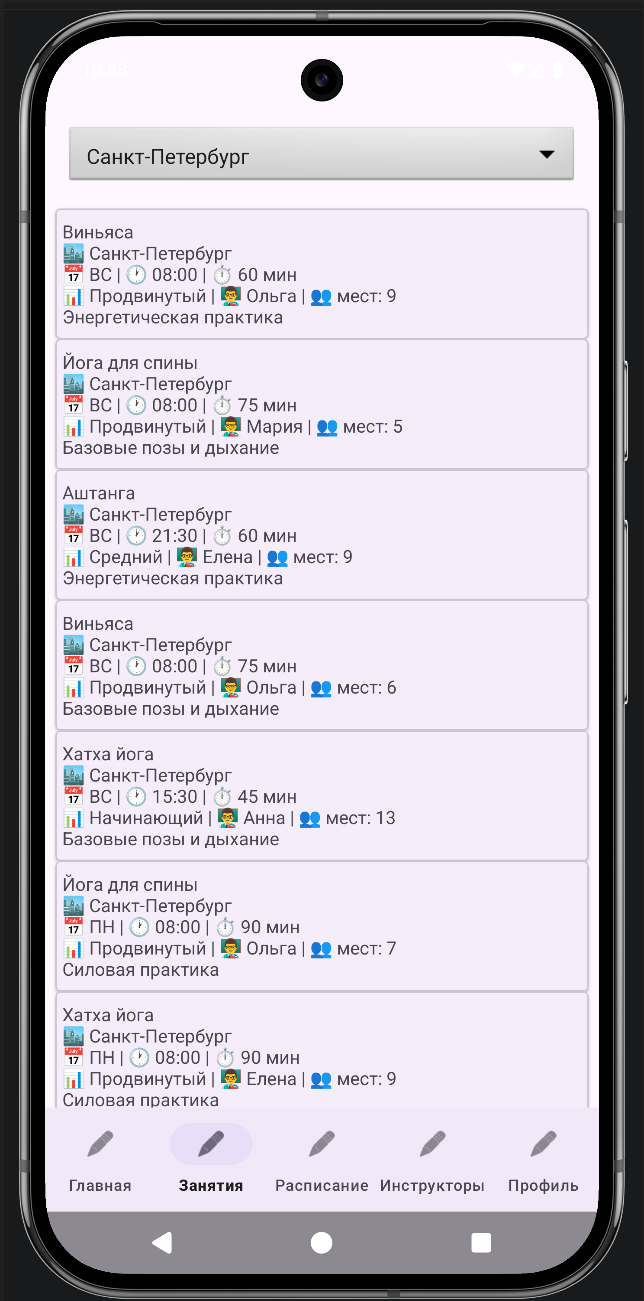
\includegraphics[width=0.4\textwidth]{images/classes.png}
	\caption{Каталог занятий}
	\label{fig:classes}
\end{figure}

\vspace{0.5cm}

\subsection{Реализация записи на занятие}

Запись на занятие реализована с проверкой наличия свободных мест. При успешной записи данные сохраняются в SharedPreferences, после чего система отправляет уведомление о подтверждении. Отмена записи удаляет соответствующий идентификатор из хранилища.

На рисунке \ref{fig:class_detail} представлен экран детальной информации о занятии с возможностью записи.

\begin{figure}[H]
	\centering
	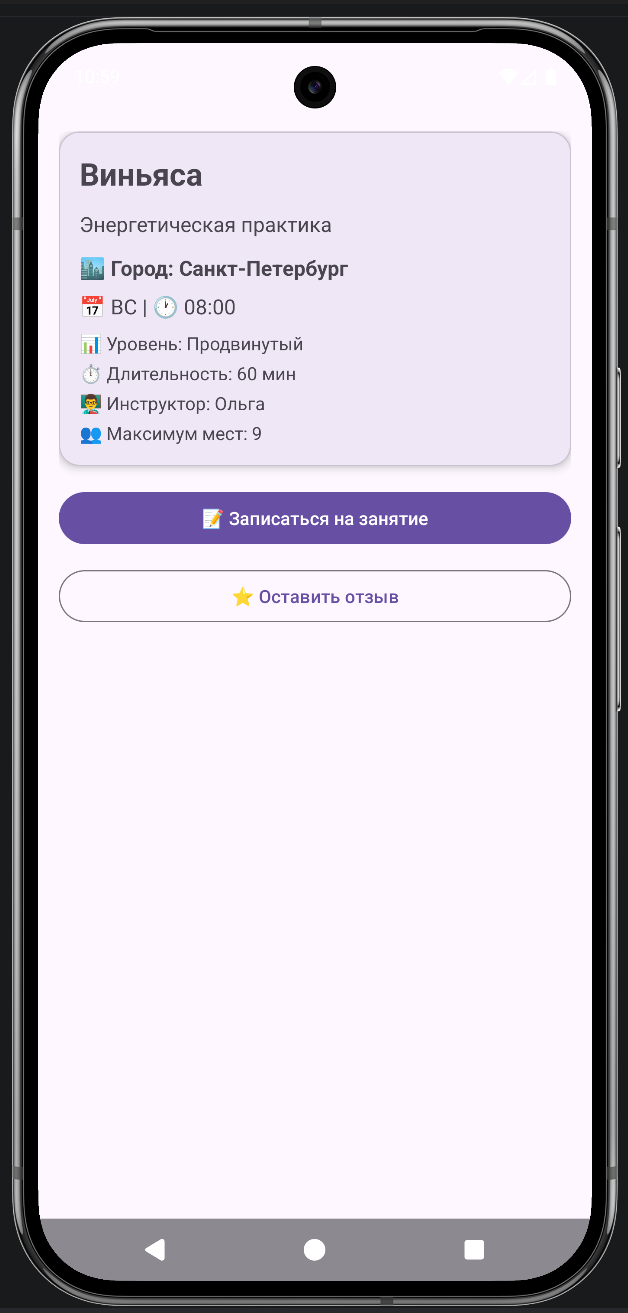
\includegraphics[width=0.4\textwidth]{images/class_detail.png}
	\caption{Детальная информация о занятии}
	\label{fig:class_detail}
\end{figure}

\vspace{0.5cm}

\subsection{Реализация расписания с календарём}

Расписание реализовано с использованием компонента CalendarView. При выборе даты система фильтрует занятия по выбранному дню и отображает список доступных занятий.

На рисунке \ref{fig:schedule} представлен экран расписания с календарём.

\begin{figure}[H]
	\centering
	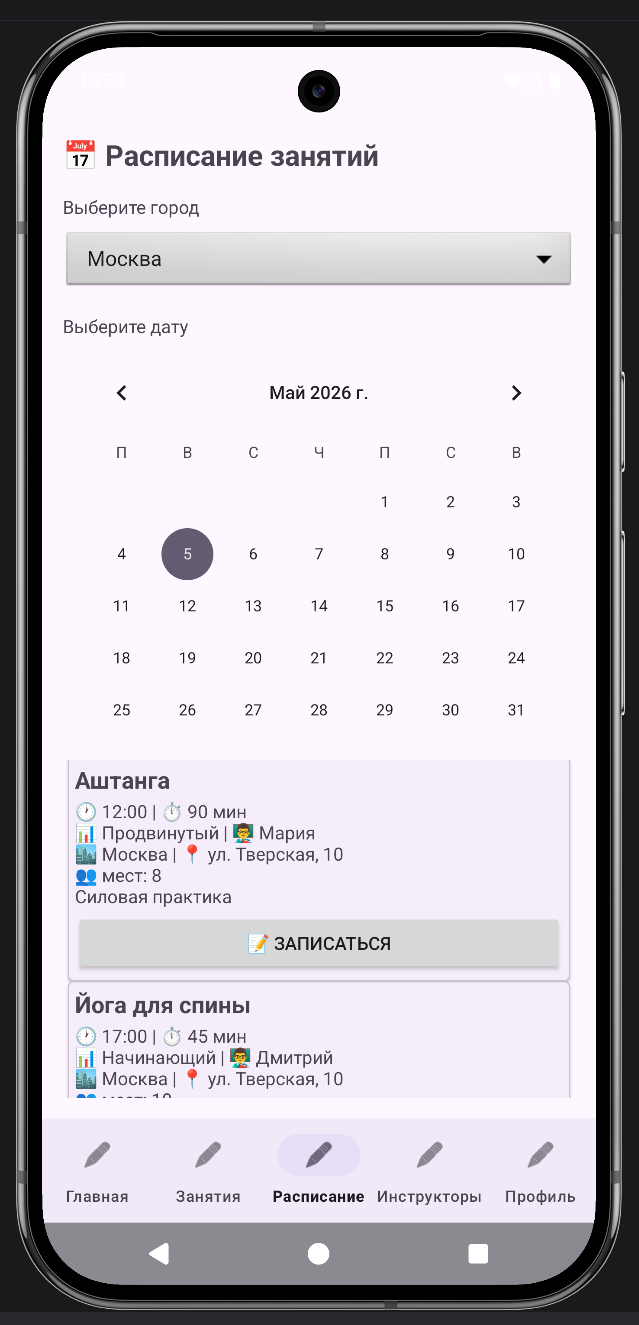
\includegraphics[width=0.4\textwidth]{images/schedule.png}
	\caption{Расписание с календарём}
	\label{fig:schedule}
\end{figure}

\vspace{0.5cm}

\subsection{Реализация профиля пользователя}

Профиль пользователя включает аватар, имя, адрес электронной почты, город и уровень подготовки. Для загрузки и отображения аватара используется библиотека CircleImageView. Все изменения сохраняются в SharedPreferences.

На рисунке \ref{fig:profile} представлен экран профиля пользователя.

\begin{figure}[H]
	\centering
	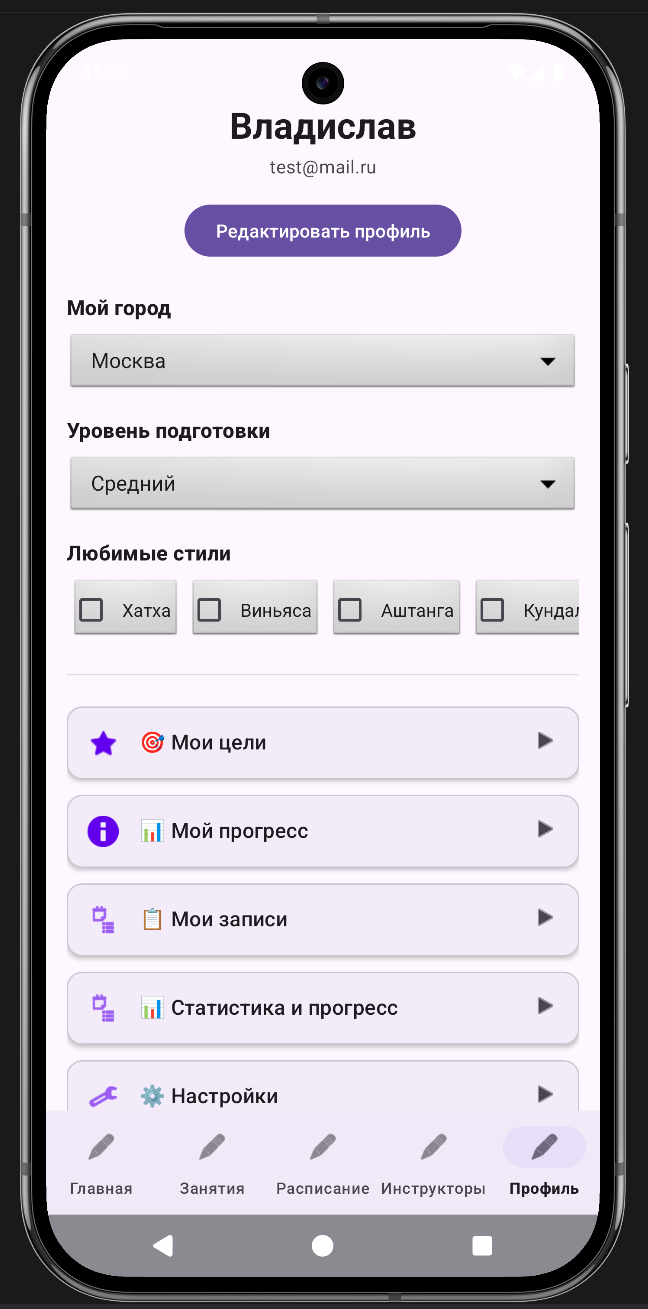
\includegraphics[width=0.4\textwidth]{images/profile.png}
	\caption{Профиль пользователя}
	\label{fig:profile}
\end{figure}

\vspace{0.5cm}

\subsection{Реализация системы отзывов и рейтинга}

Отзывы и рейтинг хранятся в SharedPreferences. Пользователь может оставить отзыв только после посещения занятия. Рейтинг отображается в виде звёзд с использованием виджета RatingBar.

На рисунке \ref{fig:review} представлен экран оставления отзыва.

\begin{figure}[H]
	\centering
	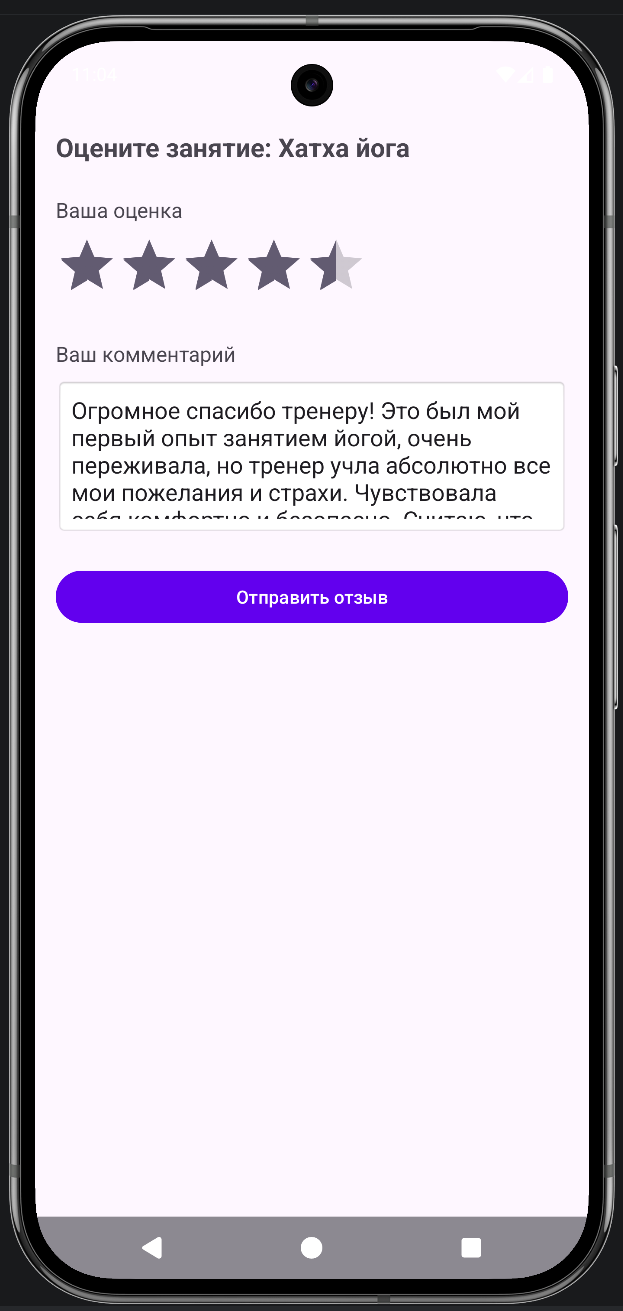
\includegraphics[width=0.4\textwidth]{images/review.png}
	\caption{Экран отзыва}
	\label{fig:review}
\end{figure}

\vspace{0.5cm}

\subsection{Реализация статистики и графиков}

Для построения графиков используется библиотека MPAndroidChart. Данные о посещениях загружаются из SharedPreferences, после чего система строит линейный график, отображающий количество занятий по месяцам.

На рисунке \ref{fig:progress} представлен экран статистики и графиков прогресса.

\begin{figure}[H]
	\centering
	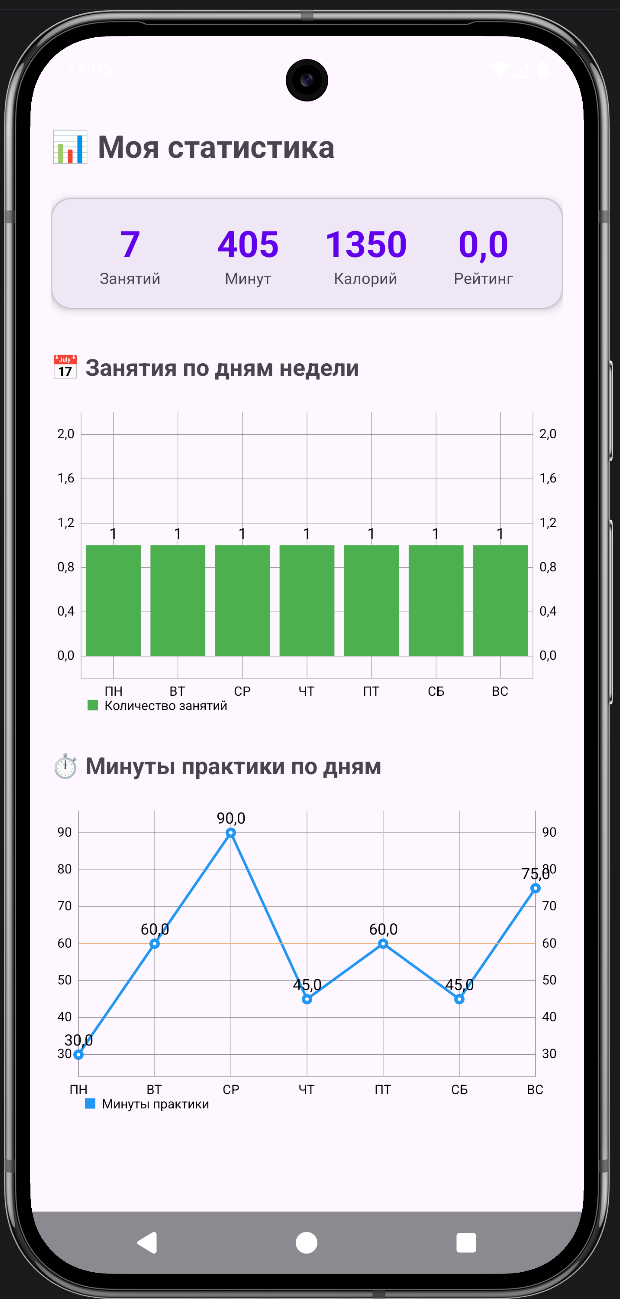
\includegraphics[width=0.4\textwidth]{images/progress.png}
	\caption{Статистика и графики прогресса}
	\label{fig:progress}
\end{figure}

\vspace{0.5cm}

\subsection{Реализация уведомлений и напоминаний}

Уведомления реализованы с использованием WorkManager для планирования напоминаний. За один час до начала занятия система отправляет push-уведомление пользователю. Уведомление о подтверждении записи отправляется сразу после успешного сохранения данных.

\subsection{Интерфейс приложения}

Пользовательский интерфейс реализован на языке разметки XML с использованием компонентов Material Design. Навигация между разделами осуществляется с помощью BottomNavigationView, который управляет загрузкой фрагментов. Все экраны приложения имеют единый стиль оформления.

На рисунке \ref{fig:home} представлен главный экран приложения.

\begin{figure}[H]
	\centering
	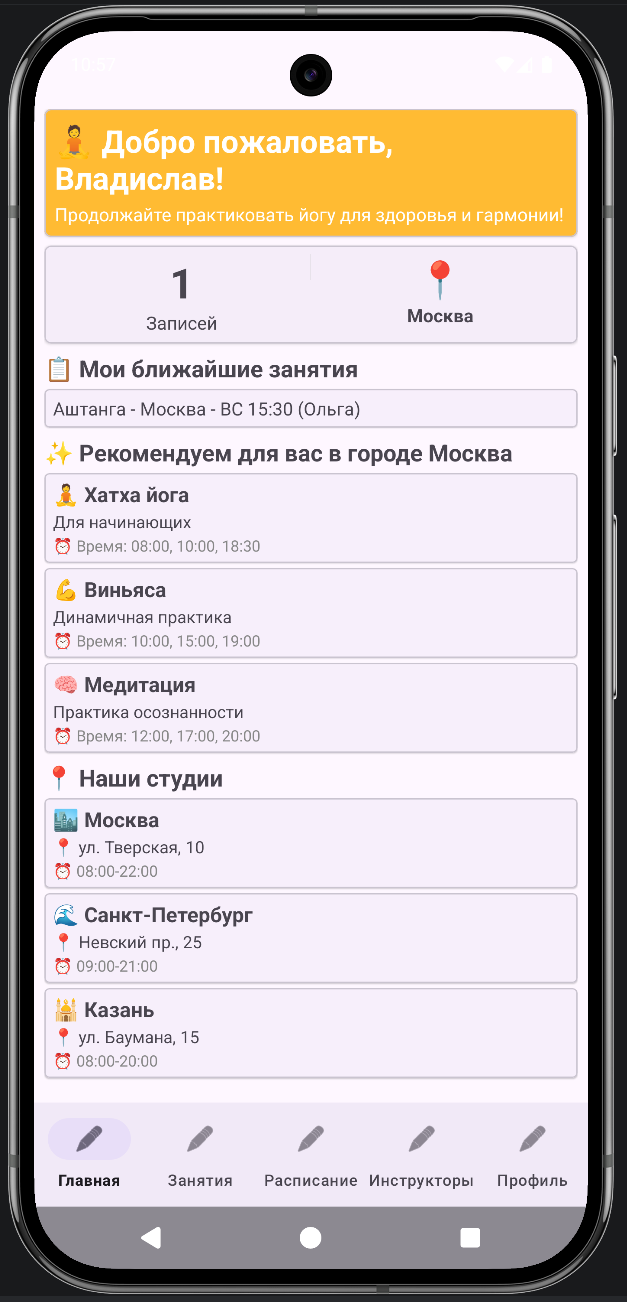
\includegraphics[width=0.4\textwidth]{images/home.png}
	\caption{Главный экран}
	\label{fig:home}
\end{figure}

\vspace{0.5cm}

На рисунке \ref{fig:instructors} представлен экран списка инструкторов.

\begin{figure}[H]
	\centering
	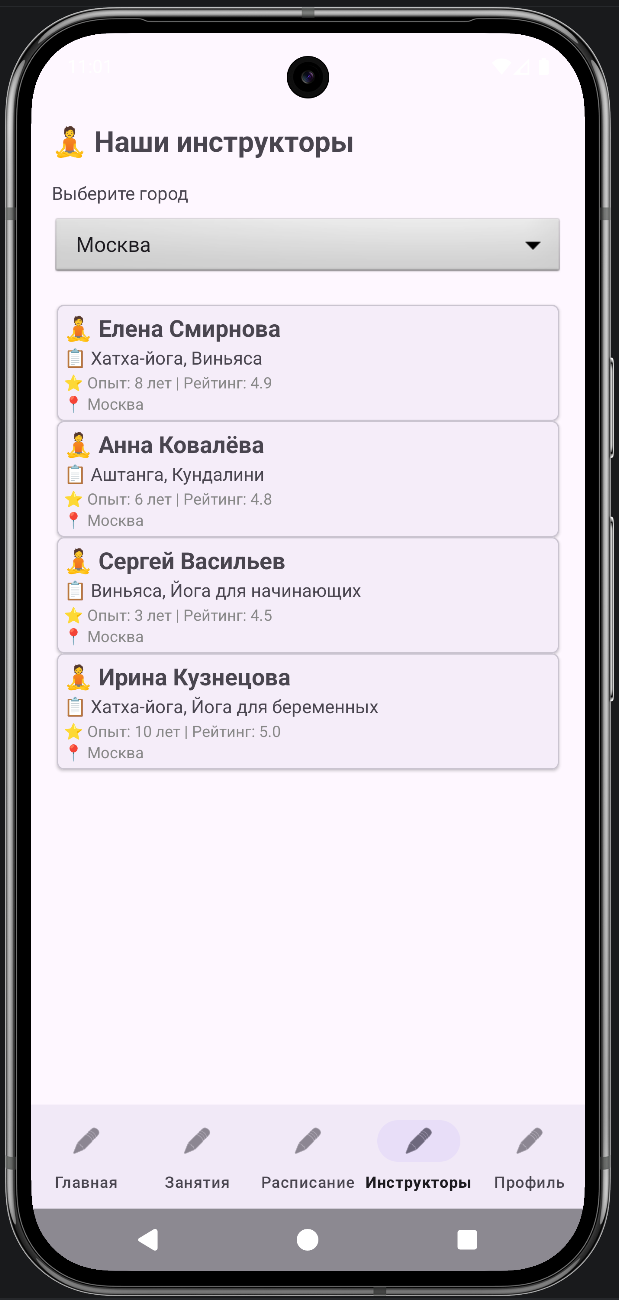
\includegraphics[width=0.4\textwidth]{images/instructors.png}
	\caption{Список инструкторов}
	\label{fig:instructors}
\end{figure}

\vspace{0.5cm}

На рисунке \ref{fig:bookings} представлен экран моих записей.

\begin{figure}[H]
	\centering
	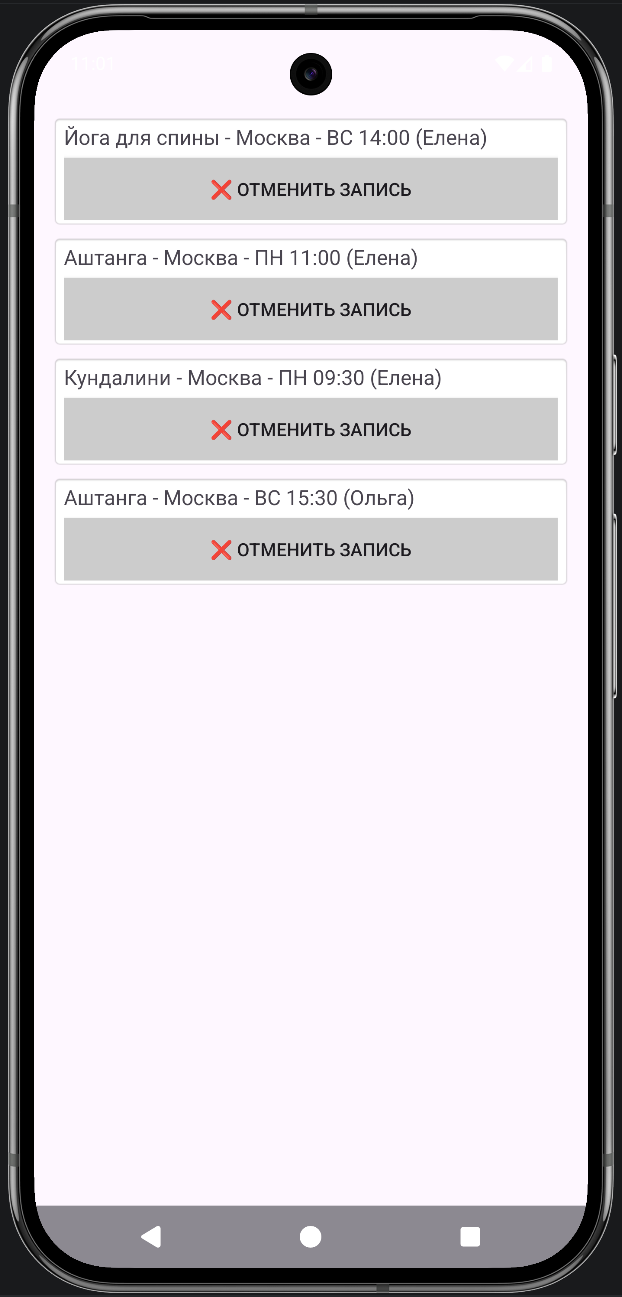
\includegraphics[width=0.4\textwidth]{images/bookings.png}
	\caption{Мои записи}
	\label{fig:bookings}
\end{figure}

\vspace{0.5cm}

\subsection{Тестирование приложения}

В ходе тестирования были проверены следующие сценарии: регистрация и авторизация пользователей, фильтрация занятий по городу, запись на занятие и отмена записи, редактирование профиля, построение графиков прогресса, оставление отзывов и рейтинга, получение уведомлений и напоминаний. Все сценарии отработали корректно.